
\section{Results}
\label{sec5:results}


Prior to damage, twenty controllers were optimized (for \mbox{$G=1500$} generations) to generate forward movement in the simulated quadruped during an evaluation period of 4 sec (with numerical integration time steps of 0.000151 sec).
Predamage displacement ranged from 37 to 46 cm (6.2 - 7.7 body lengths).

In order to isolate the effect of shape change relative to that of controller adaptation, across a diversity of insult, the simulated robot is copied $9*2*20=360$ times; once for each unique damage scenario (9 total), recovery option (2 total) and controller (20 total) triplet. 
Each copy is thus given an optimized controller and recovery option, cut according to its particular damage case, and then reoptimized for displacement (for \mbox{$G=500$} postdamage generations).
% with a unique random seed

\subsection*{The performance recovered after damage.}


Figure~\ref{fig5:recovery} plots 
mean relative performance (i.e.,~postdamage displacement as a fraction of predamage displacement),
with 99\% bootstrapped confidence intervals,
for the two recovery options in each damage scenario. 



\begin{figure}
\begin{center}
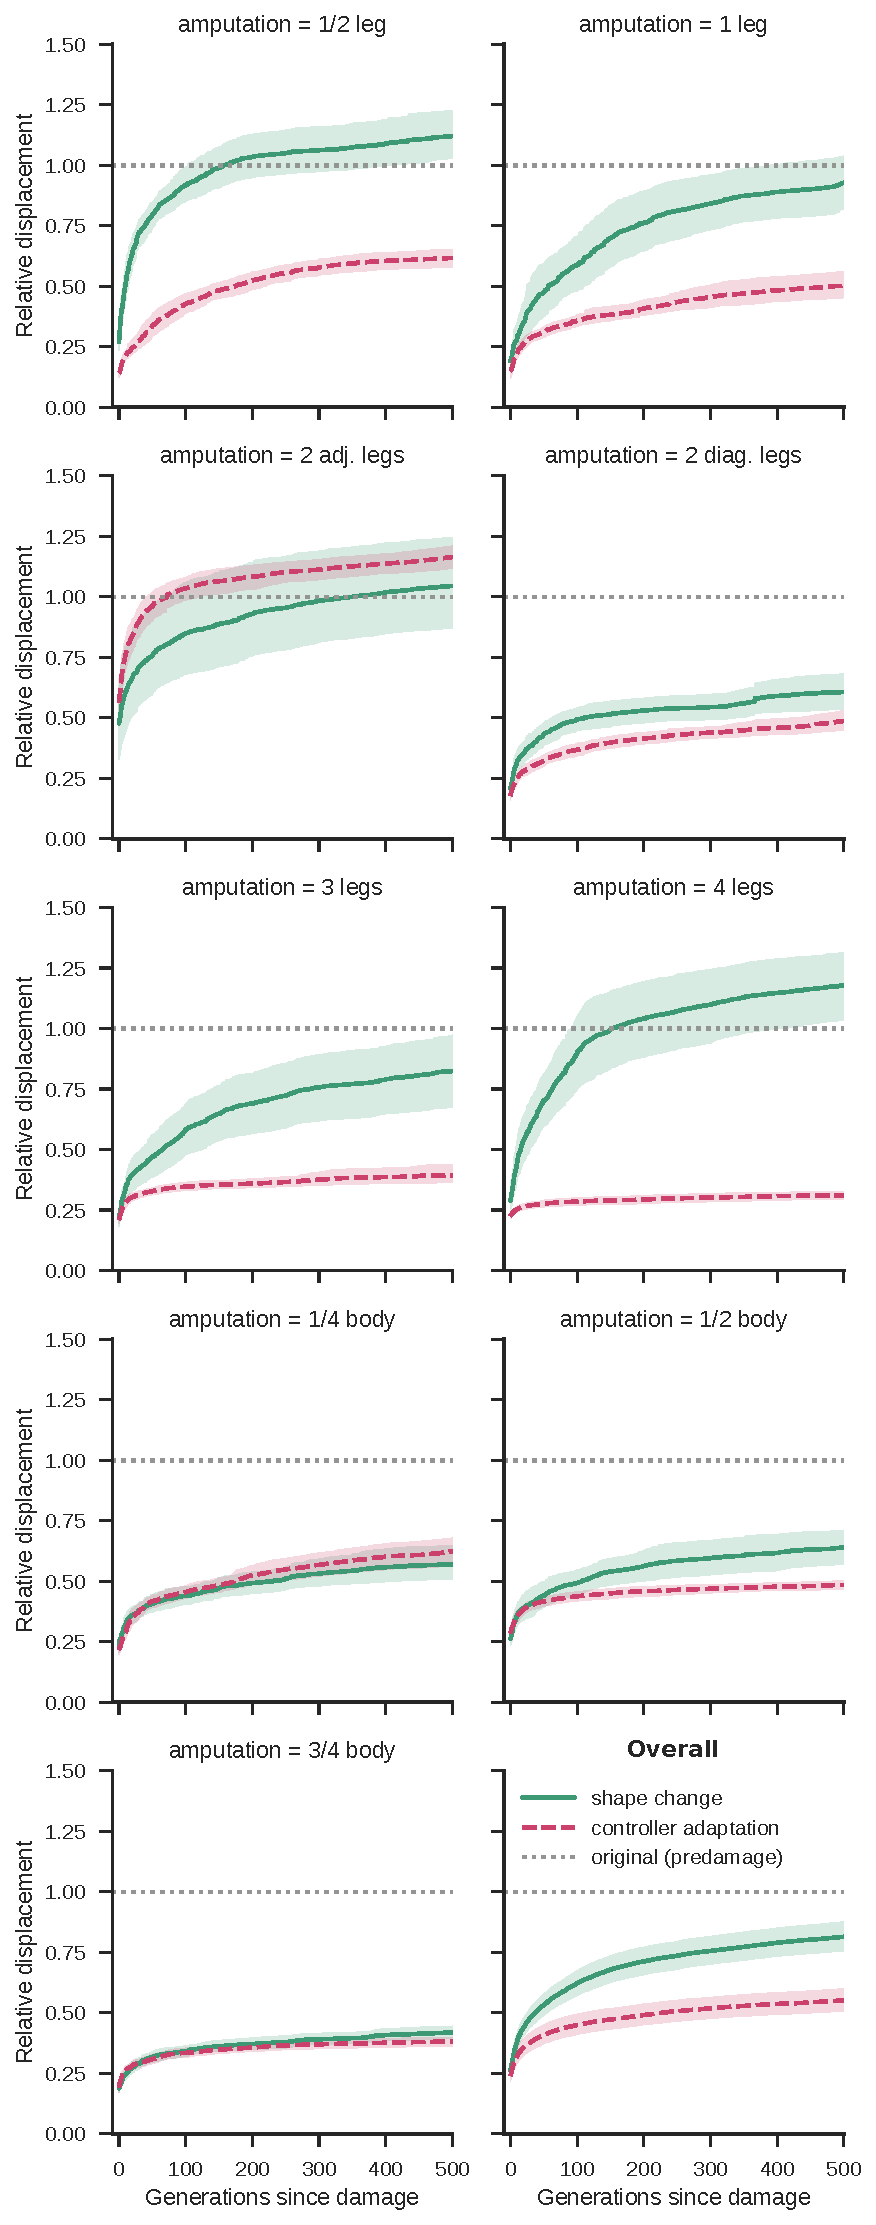
\includegraphics[width=0.5\linewidth]{Chapter05/fig/RSS_Recovery.pdf}\\
% \vspace{-3pt}
\caption{\label{fig:recovery}
Mean relative displacement (i.e.,~recovered performance) with 99\% CIs,
at each generation $(g)$ of reoptimization since damage occurred $(g=0)$.
}
\end{center}
\end{figure}

 

There are two, \textit{independent} recovery options: controller readaptation (control) and shapeshifting (treatment).
For each damage scenario,
the data consist of two random samples, a sample from the control population (20 independent trials, holding the shape of the damaged structure fixed) and an independent sample from the treatment population (20 independent shape optimization trials, holding the controller fixed).
On the basis of these samples we wish to investigate the presence of a treatment effect that results in a shift of location (median).
The null hypothesis is that of no treatment effect; 
the samples can be thought of as a single sample from one population. 

We used a distribution-free rank sum test (Wilcoxon, Mann and Whitney) for the hypothesis of no treatment effect, with Bonferroni correction for nine comparisons.
The corrected rank sum test and the 99\% bootstrapped CIs (of the mean) are in agreement.
That is, statistical significance between shapeshifting and controller adaptation, at the 0.01 level, can be correctly inferred, for each damage scenario, by visual inspection of Fig.~\ref{fig5:recovery} (i.e., no overlap in the shaded confidence intervals here implies rejection of the null hypothesis).

Overall, shape change was more successful (often better and never worse) than controller adaptation.
Interestingly, the proportion of fitness recovered was in some cases higher than one.
This could be due to a lack of volume conservation and the possibility that larger robots simply run faster than small ones.
However, many robots recovered by reducing their overall volume (e.g.,~Figs.~\ref{fig5:splay} and \ref{fig5:scruncher}).
Moreover, controller adaptation also achieved higher-than-predamage performance in one case (amp.~=~2~adj.~legs), and this phenomenon was also documented in \cite{cully2015robots} but not via shape change.

To explicitly control for the effect of body size, we optimized the controller of an otherwise identical quadruped that is twice the size of the original (Fig.~\ref{fig5:size_effect}).
Isometrically increasing volume did not affect speed: There was no significant difference in speed (at the 0.01 level) between the enlarged and original quadruped. 
This is because the controller oscillations are added on top of (not relative to) the root shape~(Eq.~\ref{eq5:beam_configuration}).
The enlarged robot has eight times the volume of the original, beam length oscillations still have the same amplitude.




\begin{figure}
\begin{center}
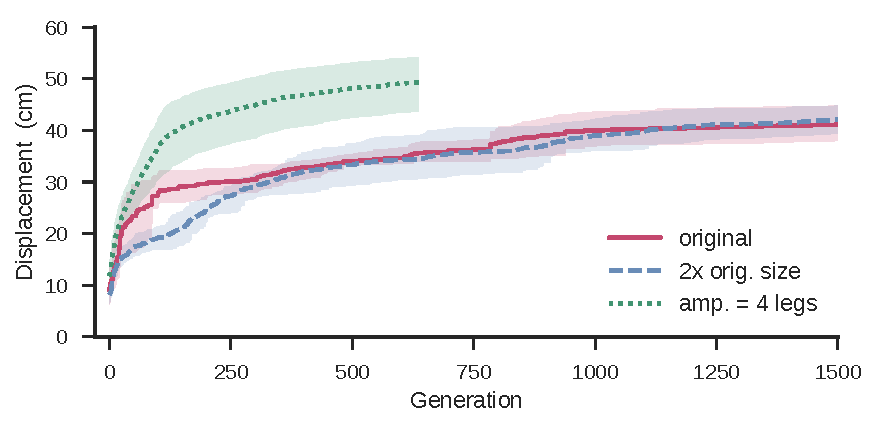
\includegraphics[trim={5pt 0 0 0},clip,width=0.7\linewidth]{Chapter05/fig/RSS_Size_Effect.pdf}\\
\vspace{-6pt}
\caption{Mean displacement with 99\% CIs of controller optimization in the predamage quadruped isometrically enlarged to maximal volume, compared to shape optimization after amputation of all four legs.
}
\label{fig5:size_effect}
\vspace{-2em}
\end{center}
\end{figure}




Despite the fact that control was optimized for the original quadruped, and that amputation of all four legs removes 23\% of the original volume and actuation (Fig.~\ref{fig5:scenarios}), robots that recovered from this particular insult through shape change (Fig.~\ref{fig5:teaser}) move significantly faster than both the original and isometrically enlarged quadrupeds (Fig.~\ref{fig5:size_effect}).
It follows that the efficacy of shapeshifting is not due simply to increased volume; rather, it is due to where and how the remnant structure's shape is deformed, which affects (e.g.) the robot's posture and mass distribution, its points of contact with the ground, and the storage and release of elastic strain energy, during locomotion.


\subsection*{The found techniques of recovery.}


We found that the optimizer discovered diverse recovery strategies through shape change (Figs.~\ref{fig5:splay}-\ref{fig5:flipper}), whereas controller readaptation often converged on the same strategy.
For example, with all four legs removed due to damage, the robot is reduced to a cuboid, and the only viable locomotion technique found by controller readaptation was crawling.
During postdamage optimization, many of these robots evolved crawling by peristalsis or in a manner that resembles the serpentine crawling of snakes \cite{alexander2003principles}.

Deforming the structure, even in a random manner, tends to produce greater frictional anisotropy which enhances peristalsis and serpentine crawling, and enables yet simpler forms of movement such as two-anchor crawling \cite{alexander2003principles}.

Nevertheless, crawling is inefficient because of drag.
Here, in many damage cases, behavioral competence was recovered through shape changes that partially or completely (but, due to material constraints, never perfectly) regenerated missing legs.
Notably, when all four legs were amputated, recovery strongly converged on the solution of regeneration, and the resulting designs were some of the fastest overall~(Fig.~\ref{fig5:teaser}).
Note that the objective function does not assume or directly select for legged locomotion.


Other amputations, however, can be beneficial, if they result in a shape that is easier to efficiently control than the original:
Prior to damage, the robot's sagittal silhouette resembles a~$\Pi$.
When two adjacent legs are amputated, the resulting $\Gamma$ shape, which initially falls forward like this \rotatebox[origin=cB]{-60}{$\Gamma$} due to gravity, tends to rapidly surpass predamage performance through controller readaptation alone, despite its diminished size.

When only half of a leg was lost to injury, some robots contracted all of the undamaged legs to recover a stable but shorter quadrupedal form.
Others seemed to simply regenerate the missing part through local volumetric expansion at the site of damage:
The stump was isometrically expanded into a leg that was the same length as the original but much wider.

On closer inspection, however, many of those who regenerated a limb also made various other compensatory shape changes away from the site of damage, such as expanding and curving their spine.
Thus even when damage is isolated to a small part of the robot's structure,
global changes, in addition to local repairs, can sometimes streamline recovery.


When damage was distributed across a wider portion of the body, a diversity of solutions were discovered.
For example, after the amputation of a quarter of the robot's body, the robot occasionally splayed out its pelvis to form a straighter and faster shape~(Fig.~\ref{fig5:splay}).
And, after the amputation of three legs, some robots once again grew replacements, but, because of other changes (e.g.,~a greatly expanded back),
the remaining ``genuine'' leg needed to be partially contracted and tucked inward for balance~(Fig.~\ref{fig5:tucker}).

\begin{figure}[h!]
\begin{center}
% \vspace{-4pt}
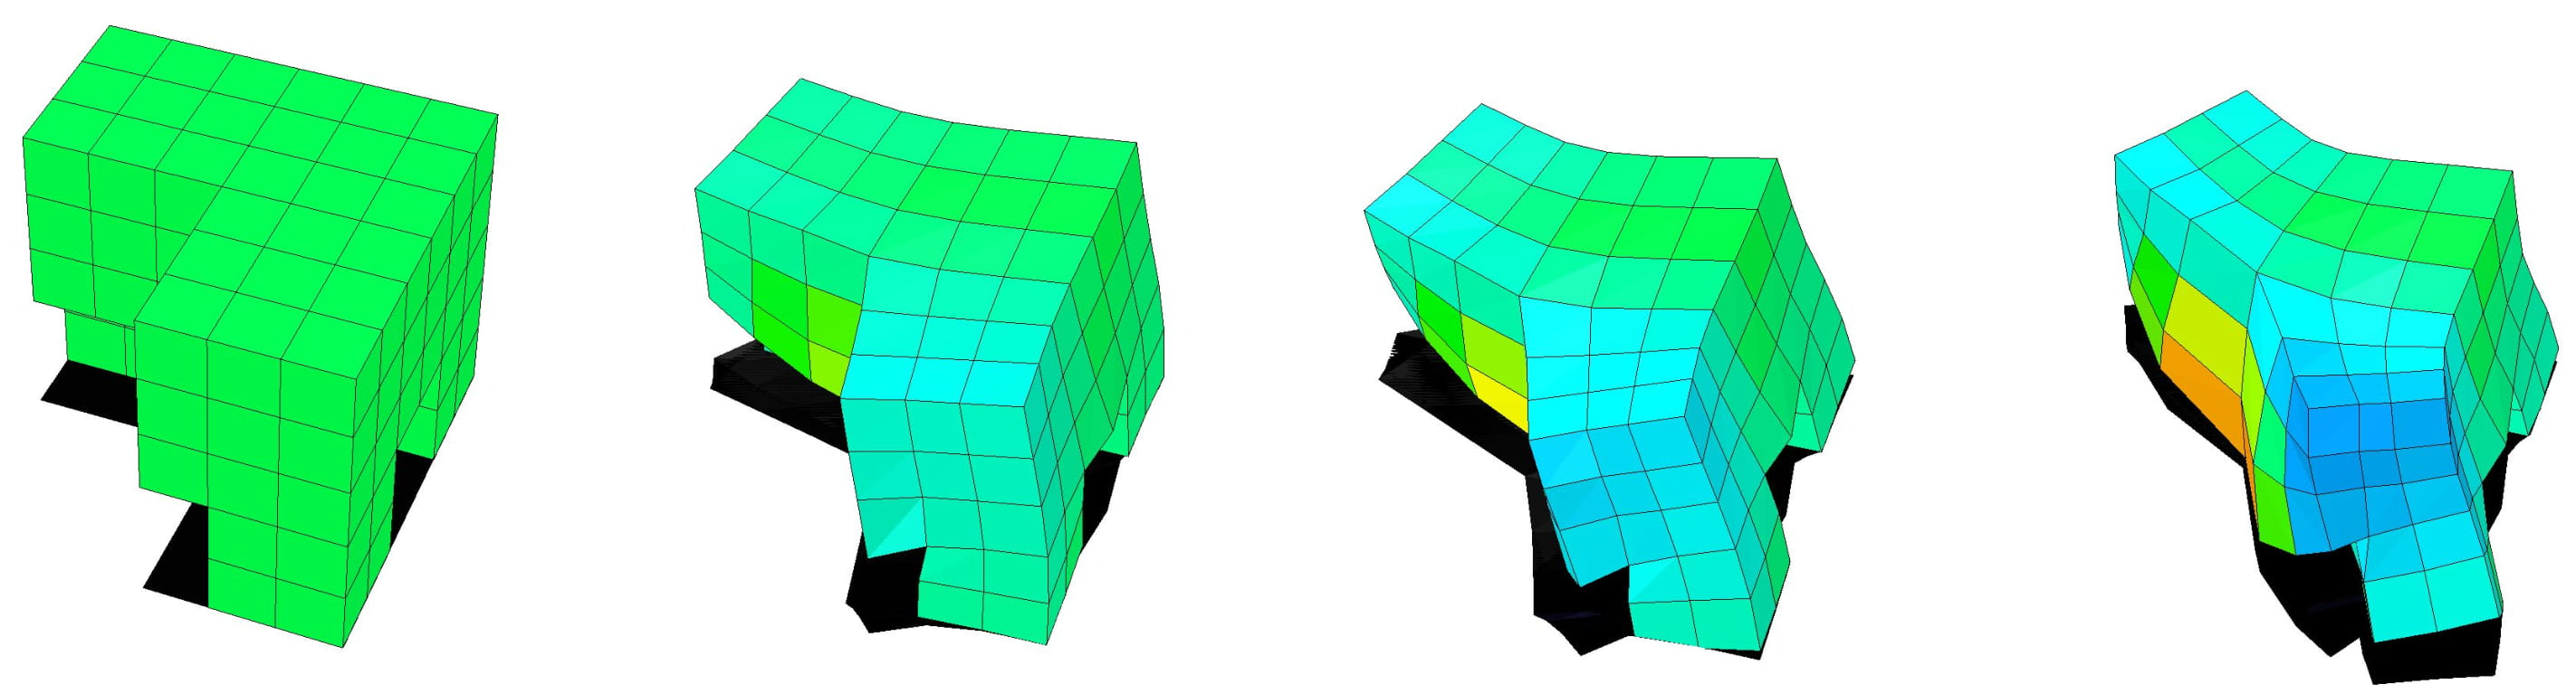
\includegraphics[trim={0 0 0 0},clip,width=\linewidth]{Chapter05/fig/splay.jpg}\\
% \vspace{-4pt}
\caption{\label{fig:splay}
This damaged robot (amp.~=~1/4~body) contracted its hips and expanded its pelvis to recover function
(\href{https://youtu.be/UBvsR6tZf5c}{\textcolor{blue}{\textbf{\texttt{youtu.be/UBvsR6tZf5c}}}}).
}
\vspace{-1em}
\end{center}
\end{figure}

In the case where half of the robot's body is removed, the undeformed structure falls under gravity onto its side; one local optima was thus to crawl ``facedown''.
A better strategy was found in which the robot could remain upright by using the two remaining limbs as forelegs and expanding the stump to form a wide hind leg.
An equally proficient strategy was observed in which the robot diminished one or both of its legs, expanded its spine, and moved longitudinally~(Fig.~\ref{fig5:scruncher}).

\begin{figure}[h!]
\begin{center}
% \vspace{-15pt}
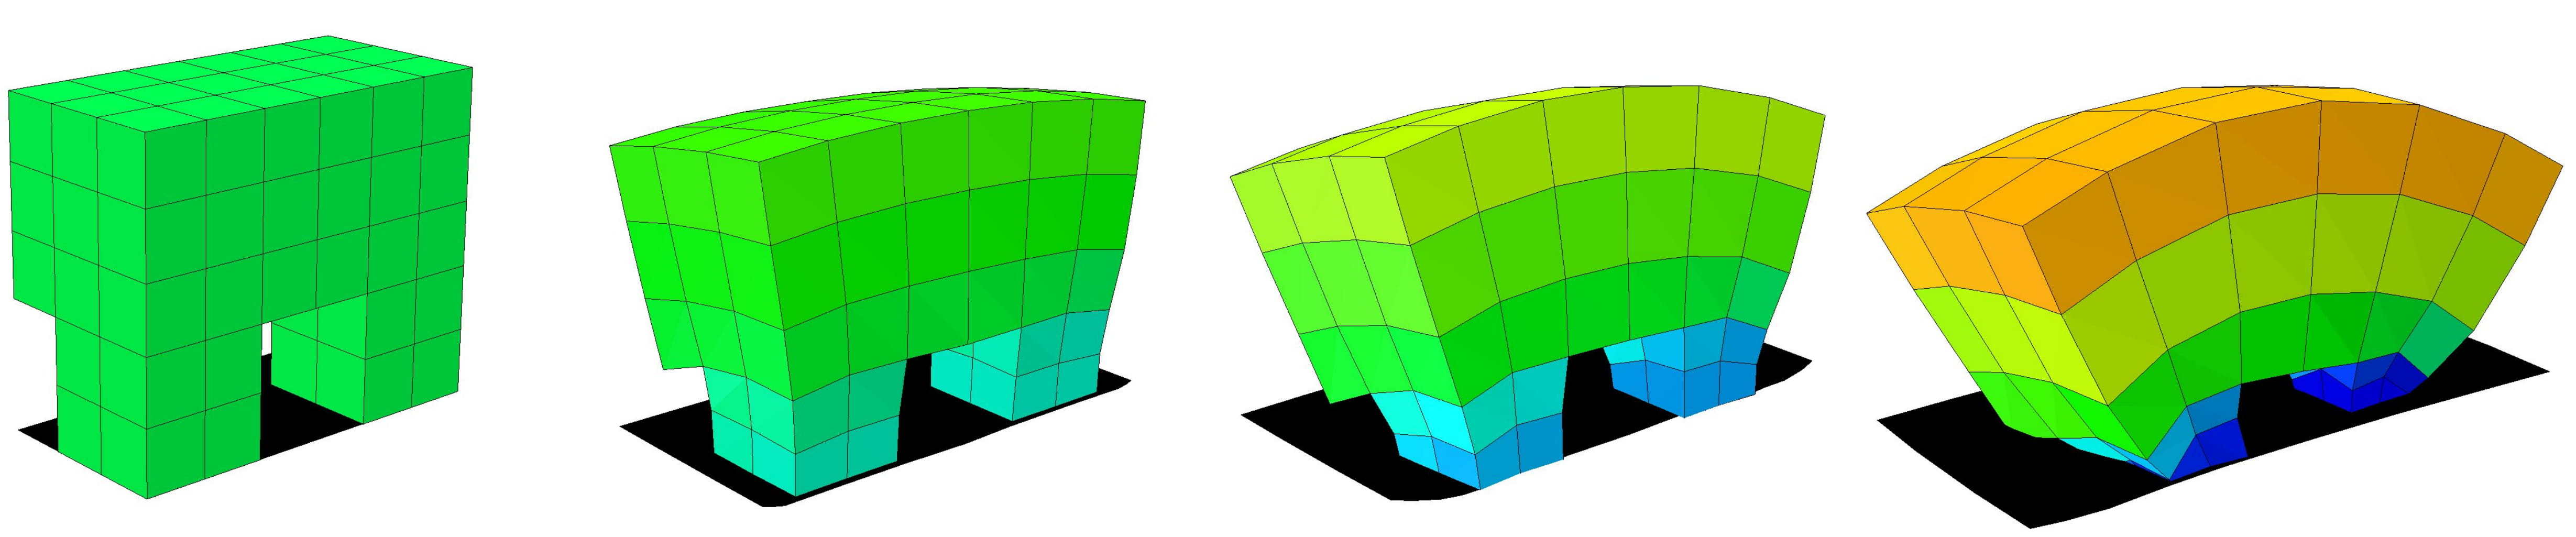
\includegraphics[trim={0 0 0 0},clip,width=\linewidth]{Chapter05/fig/scruncher.jpg}\\
% \vspace{-4pt}
\caption{\label{fig5:scruncher}
Shape change in this damage case (amp.~=~1/2~body) enabled upright, lengthwise movement, instead of falling over
(\href{https://youtu.be/nfCaVZVBmKI}{\textcolor{blue}{\textbf{\texttt{youtu.be/nfCaVZVBmKI}}}}).
}
\vspace{-1em}
\end{center}
\end{figure}


There were many successful variations on this theme,
but one of the best designs in this case did the exact opposite: The robot expanded its remaining limbs to their maximum volume, contracted its spine, and flipped over (once) to walk longitudinally with the added momentum generated from large, swaying front and back limbs~(Fig.~\ref{fig5:flipper}).


\begin{figure}[h!]
\begin{center}
% \vspace{-15pt}
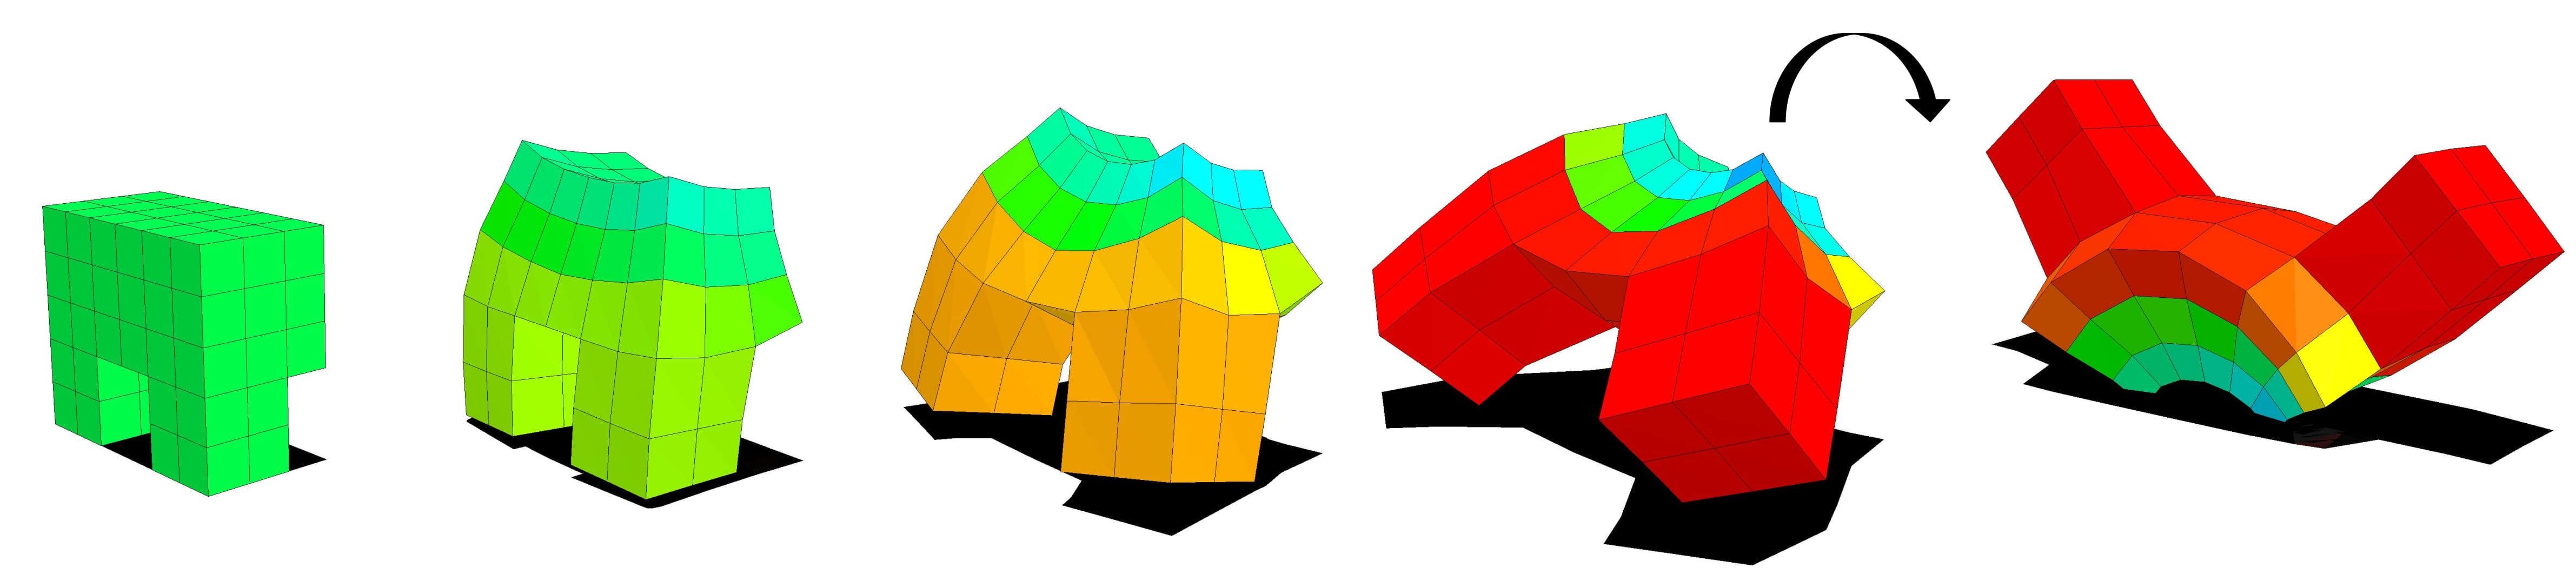
\includegraphics[trim={0 0 0 0},clip,width=\linewidth]{Chapter05/fig/Flipper2.jpg}\\
% \vspace{-5pt}
\caption{\label{fig:flipper}
This damaged robot (amp.~=~1/2~body) contracted its spine, expanded its limbs, and flipped over onto its back to walk lengthwise and exploit the elastic properties of its new arms
(\href{https://youtu.be/WwYdSnuJBBA}{\textcolor{blue}{\textbf{\texttt{youtu.be/WwYdSnuJBBA}}}}).
}
\vspace{-1em}
\end{center}
\end{figure}

However, after the most extreme insult, when all but a quarter of the robot is lost, there is insufficient material to regenerate legs or execute other more extreme shape changes. 
Neither recovery option cultivated (visually) appreciable gains in fitness.
Yet, while this case removes 71\% of the original volume it is significantly \textit{less} deleterious to controller optimization than amputating the four legs, which removes just 23\% of the original volume.
Insult is thus a matter of kind, not degree.


\subsection*{The transferal of recovery strategies to reality.}


To investigate the potential for directly transferring recovery strategies from simulation to reality, we aimed to transfer the overall shapes that are pictured in Figs.~\ref{fig5:teaser} and~\ref{fig5:tucker}. 
In these particular cases, the optimizer found shapes with contiguous sections of voxels actuated to similar levels. 
Thus, we here examine the one-actuator case, in which the voxels with the largest rest volumes---the top layer of ($6\times6=36$) voxels and the two corner voxels just below the top layer, on each corner of the torso (8 in total)---were connected to the same air inlet. 
Voxels not hooked into the air line were punctured to allow for passive deflation and contraction of the robot, mimicking the simulated robot's ability to contract voxels by decreasing the rest lengths~$b_i$. 



\begin{figure*}
\begin{center}
% \vspace{-6pt}
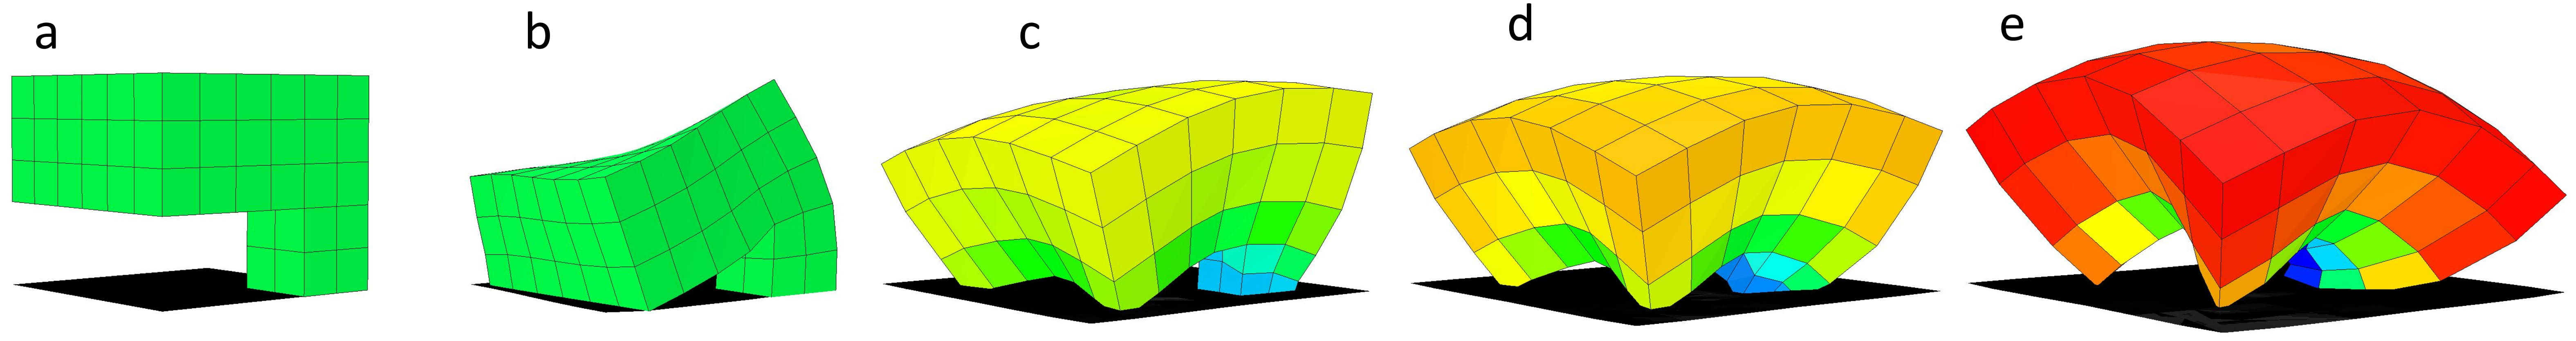
\includegraphics[trim={-40pt 0 0 0},clip,width=\linewidth]{Chapter05/fig/tucker.jpg} \\
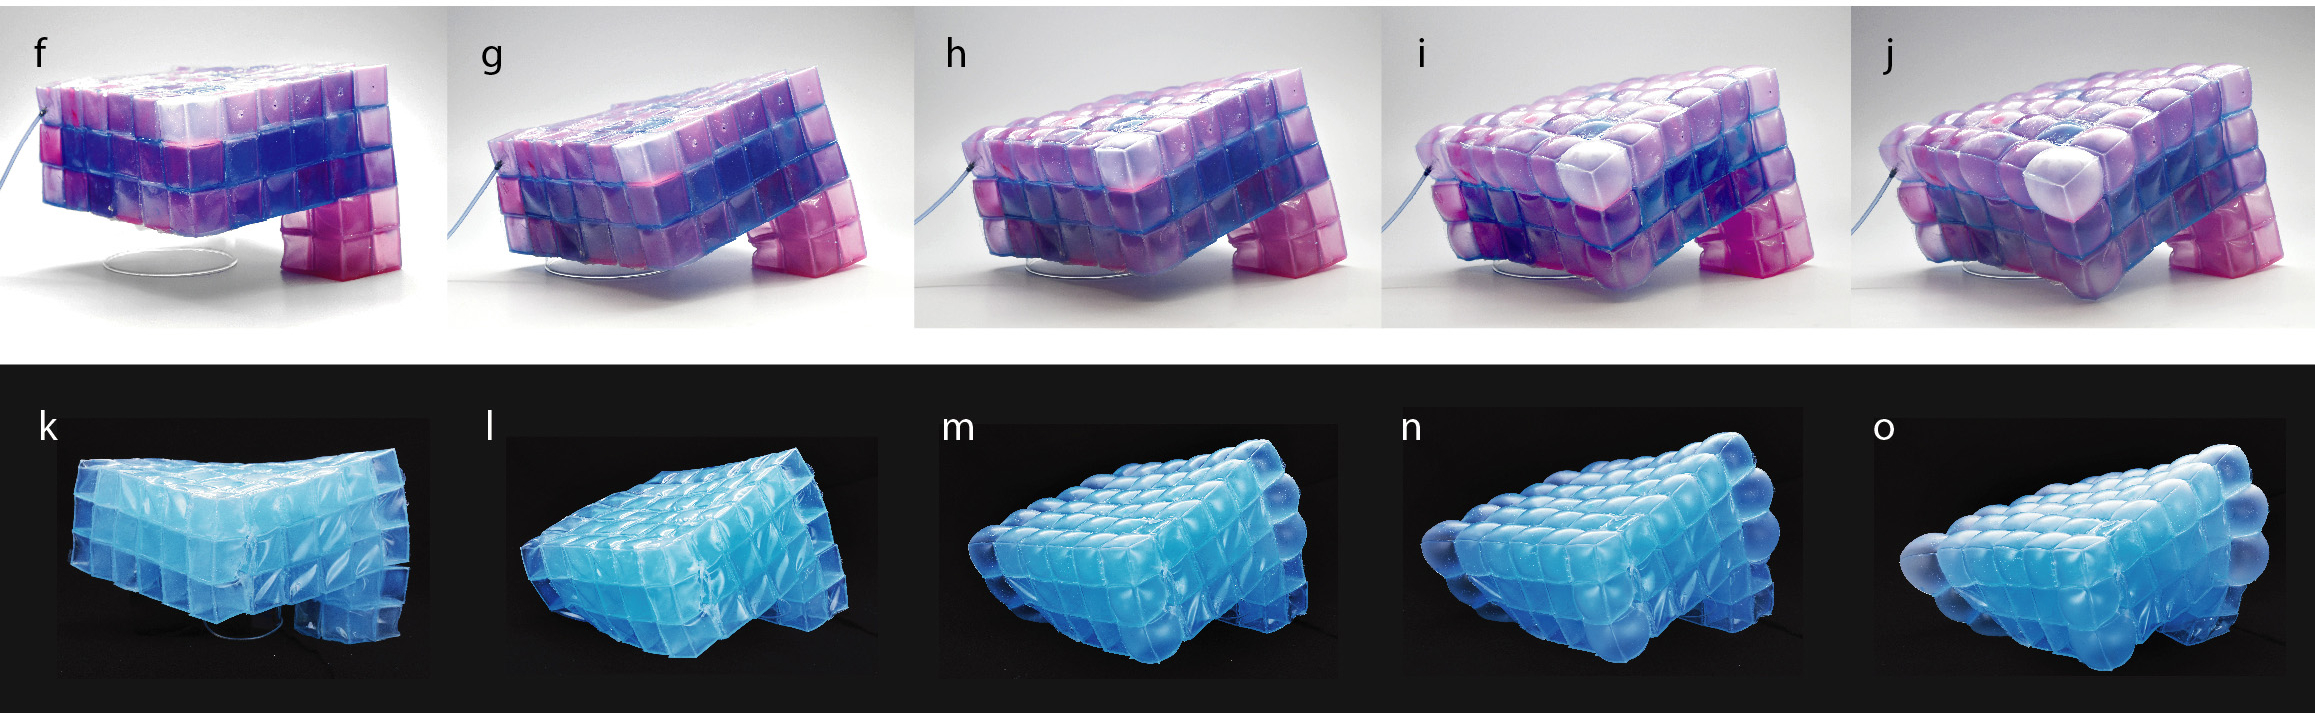
\includegraphics[trim={0 0 0 -5pt},clip,width=\linewidth]{Chapter05/fig/VoxelBotTuckerCropped.jpg}\\
% \vspace{-2pt}
\caption{\label{fig:tucker}After losing three legs to injury (amp.~=~3~legs), the former quadruped is reduced to a monopedal structure~(\textbf{a}), the shape of which was then optimized for locomotion speed, resulting in an expanded spine, the folding-inward of the remnant predamage leg, and the ``regeneration'' of the three missing legs~(\textbf{c-e}).
This simulated strategy was then realized in two implementations using pneumatically-actuated, cubic elastomer bladders. The purple robot~(\textbf{f-j}) consists of two layers of drip-molded silicone; the blue robot~(\textbf{k-o}) consists of a single layer, and is thus less stable but more deformable.
A single air inlet here yields the rudiments of appropriate shape change, but pressure oscillations in this setup did not yield locomotion
(\href{https://youtu.be/A2KTGhCFxK8}{\textcolor{blue}{\textbf{\texttt{youtu.be/A2KTGhCFxK8}}}}).
}
% \vspace{-2em}
\end{center}
\end{figure*}

The purple robot adequately expands the top layer of voxels in both cases (Figs.~\ref{fig5:teaser}j and~\ref{fig5:tucker}j), but fails to reach the overall target shapes drawn in Figs.~\ref{fig5:teaser}e and~\ref{fig5:tucker}e. 
Although further increasing pressure did indeed lead to larger deformations,
the outer voxels inflate farther than interior ones, limiting the maximum viable actuation pressure. 
The thinner voxel walls of the blue robot exacerbated this issue~\mbox{(Fig.~\ref{fig5:tucker}k-o)}, 
but their increased flexibility enabled a more faithful transferal of overall surface curvature.
Another limitation we discovered was friction.
Fully realizing the target shape in Fig.~\ref{fig5:tucker}e requires the robot to drag its leg inward across the floor, tucking it under its body; but the silicone leg often stuck to the surface, preventing the prescribed maneuver in reality.


The silicone design and 1-axis rotational molding technique are still quite promising. 
Even when inflated at high enough pressures to make the outer voxels approximately spherical (Fig.~\ref{fig5:tucker}o), the voxels did not rupture. 
To achieve more consistent expansion of interior and exterior voxels, the later should be inflated at a lower pressure than the former.
By incorporating strain sensors \cite{white_low-cost_2017} and closed-loop control in future, the robot could correct for this variation on the fly.
By actuating different voxels at different pressures, and enabling active contraction in addition to expansion, a much wider range of simulated shapes could be attained in reality. 

